\section{Case Study}
In this section, we show how we adopt several commonly used scientific workflows in Beeflow. We first analysis the dependency mode of each task in each workflow. Then, we determine the data flow mode between each tasks. Finally, we construct DAG for each workflow, which can be used for configuring Beeflow.
\subsection{VPIC Workflow}
VPIC is a general purpose particle-in-cell simulation code for modeling kinetic plasmas in one, two, or three spatial dimensions \cite{bowers20080, bowers2008ultrahigh, bowers2009advances}. In our VPIC workflow, we perform turbulence simulation on VPIC. As VPIC is running, it dumps output data files, which will be read by ParaView Server \cite{ahrens2005paraview, ayachit2015paraview}. ParaView is an open-source, multi-platform data analysis and visualization application. ParaView users can quickly build visualizations to analyze their data using qualitative and quantitative techniques. ParaView toolkit has two parts: ParaView Server and ParaView Client. ParaView Server is mainly responsible for communicate, control and gathering data from scientific applications. ParaView Client usually runs on users local machines and responsible for visualize scientific data by connecting with ParaView Server. One common use case is run ParaView Server on the same platform as scientific application at the same time, and also run ParaView Client on local machine to monitor simulation process by receiving rendering data from ParaView Server. This is also the use case in our VPIC workflow as shown in \textbf{Figure \ref{vpic-wf}}. 
\begin{figure}[h]
    \centering
    \caption{VPIC workflow}
    \label{vpic-wf}
    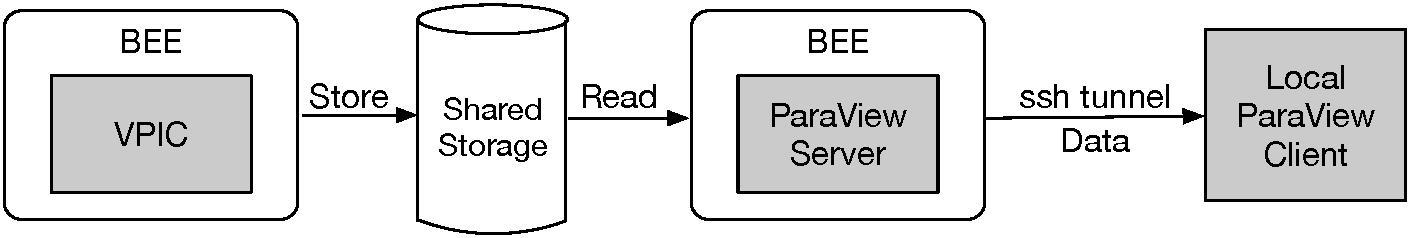
\includegraphics[width=0.5\textwidth]{figures/vpic.pdf}
\end{figure}
To launch VPIC workflow with Beeflow, we first analysis the tasks in it. Since only VPIC and ParaView Server need to run on computing nodes, only those two need to be handled by BEE. ParaView Server can read and process data while VPIC is dumping data, so those two tasks are in in-situ dependency mode, which need to be configured in Beeflow description file. Also, those two tasks use disk-based data sharing, so BEE need to be configured so that they mount the same directory/EFS on targeting platform. The abstracted DAG can be represented as \textbf{Figure \ref{vpic-dag}}
\begin{figure}[h]
    \centering
    \caption{DAG of VPIC workflow}
    \label{vpic-dag}
    \includegraphics[width=0.5\textwidth]{figures/vpic-beeflow.pdf}
\end{figure}

\subsection{Flecsale Workflow}
Flecsale \cite{flecsale} is another workflow similar the previous VPIC workflow. There are also three parts in this workflow: Flecsale, ParaView Server, and ParaView Client. There are two differences. First, instead of using VPIC, we use Flecslae, which is a computer software package developed for studying problems that can be characterized using continuum dynamics, such as fluid flow. Second, we build Flecsale with Catalyst so that it can enable network-based in-situ analysis with simulation control from ParaView. The connect here is established using previous mentioned SSH tunnel. The workflow is shown in \textbf{Figure \ref{flecsale-wf}}.

\begin{figure}[h]
    \centering
    \caption{Flecsale workflow}
    \label{flecsale-wf}
    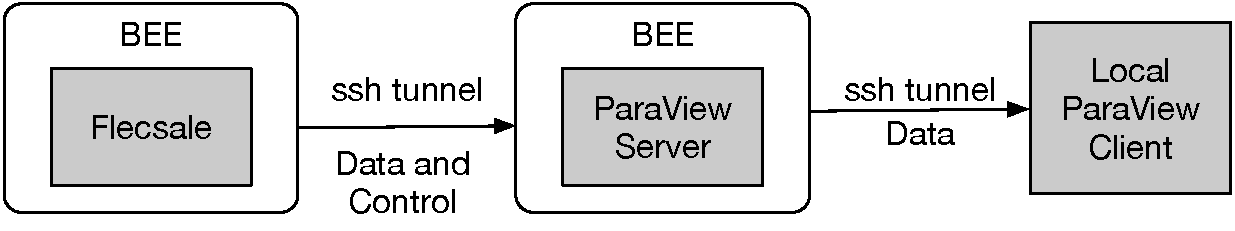
\includegraphics[width=0.5\textwidth]{figures/flecsale.pdf}
\end{figure}

By modifying the simulation application from VPIC to Flecsale and enabling SSH tunnel for BEE task containing Flecsale, we can construct the DAG for this Flecsale workflow as in \textbf{Figure \ref{fecsale-dag}}.

\begin{figure}[h]
    \centering
    \caption{DAG of Flecsale workflow}
    \label{fecsale-dag}
    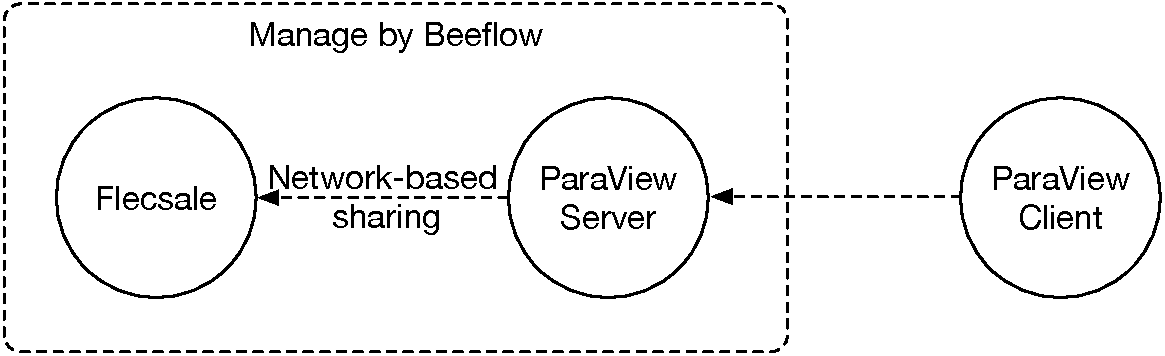
\includegraphics[width=0.5\textwidth]{figures/flecsale-beeflow.pdf}
\end{figure}

\subsection{BLAST Workflow}
In our third workflow case study, we choose a traditional BLAST workflow for DNA sequence matching. BLAST is biological application aimed to find similarity between biological sequences \cite{altschul1990basic}. In our BLAST workflow, it first let a DNA splitter divide the large-sized input DNA sequences in to several partition. Then, it launches several BLAST worker to work on one partition each. Finally, when all workers have done their job, a result collecting worker gather all results from each worker into one file. The workflow is shown in \textbf{Figure \ref{blast-wf}}.

\begin{figure}[h]
    \centering
    \caption{BLAST workflow}
    \label{blast-wf}
    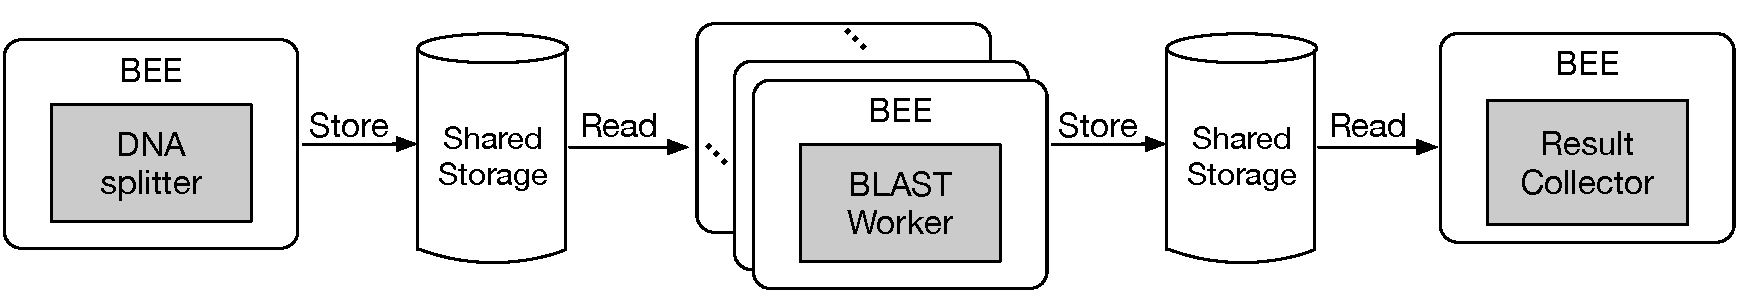
\includegraphics[width=0.5\textwidth]{figures/blast.pdf}
\end{figure}    

Next, we analysis the dependencies in this workflow. First, the DNA splitter has no depending task, so it can start as soon as we start the workflow. Then, all workers must wait for the splitter, so this is off=line dependency. Finally, the result collector needs to wait for all workers, so this is also off-line dependency. All intermedian data are share with files on disk, so all dependecies are using disk-based shareing. The DAG of this workflow can be shown in \textbf{Figure \ref{blast-dag}}.

\begin{figure}[h]
    \centering
    \caption{DAG of BLAST workflow}
    \label{blast-dag}
    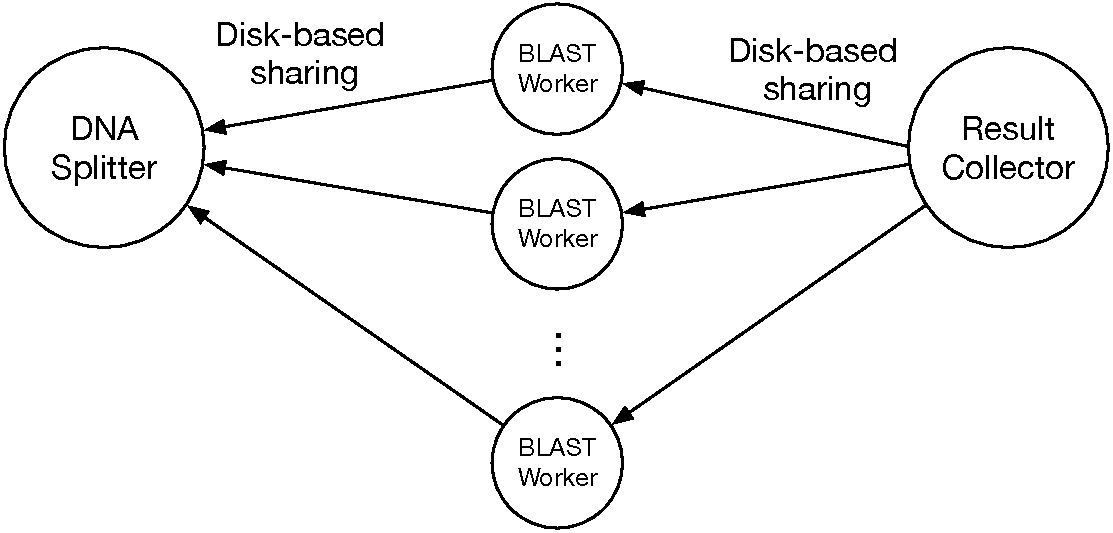
\includegraphics[width=0.5\textwidth]{figures/blast-dag.pdf}
\end{figure}



